
\section{Algorithm}

\begin{frame}{Working}
\begin{itemize}
\item[$\bullet$]Endpoints sorted
\item[$\bullet$]Intervals ordered by increasing right endpoint $\mathrm{I_{1}, I_{2},\dots,  I_{n}}$
\item[$\bullet$]Intervals processed in order using Greedy approach
\end{itemize}
\end{frame}

\begin{frame}{Processing an interval}

\begin{overlayarea}{\textwidth}{\textheight}
\vspace{0.5cm}
Two possibilities :
\begin{itemize}
\item[$\bullet$]If no available color, discard
\item[$\bullet$]Otherwise, assign best fitting color
\end{itemize}

Intuitively, best fit = closest available color on left-side

\vspace{2cm}

\only<2>{
    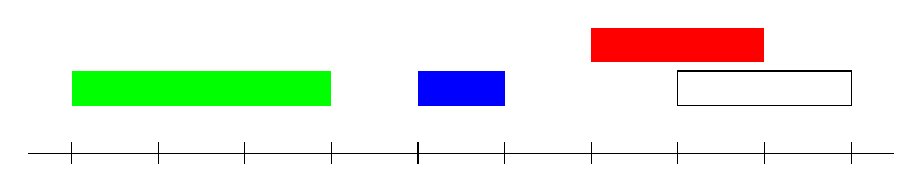
\begin{tikzpicture}[scale=0.55]
    \draw (-1,-1.5) -- (19,-1.5);
          \foreach \x in {0,2,...,18}
        {\draw (\x,-1.75) -- (\x, -1.25);}
    \fill[color=green] (0,-0.4) rectangle (6,0.4);
    \fill[color=blue] (8,-0.4) rectangle (10,0.4);
    \draw (14,-0.4) rectangle (18,0.4);
    \fill[color=red] (12,0.6) rectangle (16,1.40);
    \end{tikzpicture}
}

\only<3>{
    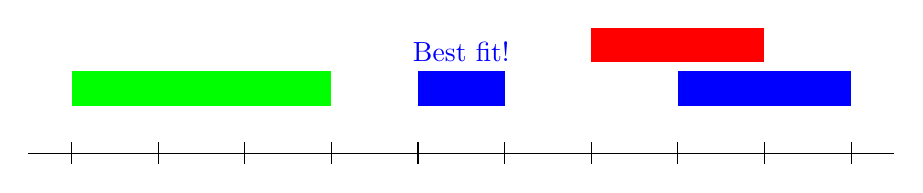
\begin{tikzpicture}[scale=0.55]
    \draw (-1,-1.5) -- (19,-1.5);
          \foreach \x in {0,2,...,18}
        {\draw (\x,-1.75) -- (\x, -1.25);}
    \fill[color=green] (0,-0.4) rectangle (6,0.4);
    \fill[color=blue] (8,-0.4) rectangle (10,0.4);
    \draw (9,0.4) node[above] {\textcolor{blue}{Best fit!}};
    \fill[color=blue] (14,-0.4) rectangle (18,0.4);
    \fill[color=red] (12,0.6) rectangle (16,1.40);
    \end{tikzpicture}
}

\end{overlayarea}
\end{frame}

\begin{frame}{Best fit}
\begin{definition}

%\vspace{0.3cm}
\textcolor{blue}{Leader} (color $\mathrm{k}$) : Interval of largest right endpoint with color $\mathrm{k}$\\

%\vspace{0.5cm}
\textcolor{blue}{Adjacent} (interval $\mathrm{I_{i}}$) : Interval of greatest right endpoint no greater than $\mathrm{I_{i}}$'s left endpoint\\

%\vspace{0.5cm}
\textcolor{blue}{Best fit leader} (interval $\mathrm{I_{i}}$) : Leader of greatest right endpoint no greater than $\mathrm{I_{i}}$'s left endpoint
\end{definition}

Best fit color for $\mathrm{I_{i}}$ = color Best\_fit\_leader($I_{i}$)

%TODO : rajouter que le best fit leader se trouve en O(1) en amortized complexity analysis
\end{frame}

\begin{frame}{Interval sets}
  \begin{itemize}
    %\item[$\bullet$]Grouping intervals by sets representing equivalence classes with respect to "best fits"
    \item[$\bullet$]Interval of least index gives its name to the set. In fact, it's a leader
    \item[$\bullet$]At any time, only 1 leader per set
    \item[$\bullet$]\texttt{find($\mathrm{I}$)} : returns the leader of the set of $\mathrm{I}$
    \item[$\bullet$]Best fit leader : \texttt{find(adjacent($\mathrm{I}$))}
\item[$\bullet$]During the algorithm : unions of sets
    %\item[$\bullet$]Processing : \texttt{if} $\mathrm{I_{j}}$ is discarded \textbf{or} not a leader, \texttt{then} set($\mathrm{I_{j}}$) $\cup$ set($\mathrm{I_{j-1}}$)
    \item[$\bullet$]Initially : singleton sets
  \end{itemize}
\end{frame}